\section{Getting started}
\label{sec:getting-started}

To begin with, we will setup our environment in order to be prepared for the upcoming exercises.

\subsection{Installing the VMs}

First, a fresh installation of VirtualBox (version \texttt{>=6.1.22}) with Oracle VM VirtualBox Extension Pack is required. The tool is completely free, open source and available for all platforms. It can be downloaded from the official website\footnote{\url{https://www.virtualbox.org/wiki/Downloads}}, where step-by-step installation instructions do follow.

\subsubsection{With the \texttt{ova} file}
\label{subsubsec:getting-started:with-ova}

If the group-provided \texttt{ova} file is available, the setup is very simple. 

Once VirtualBox is successfully installed along with (\textit{important!}) the Oracle VM VirtualBox Extension Pack, we can proceed to the import of the \texttt{ova} file. Press the button as shown in Figure \ref{fig:getting-started:import-button}.

\begin{figure}[htbp]
	\centering
	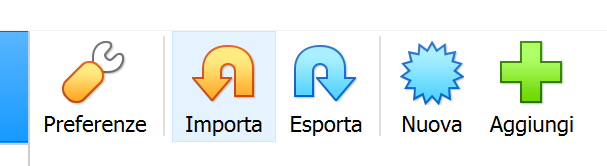
\includegraphics[width=0.4\textwidth]{../drawable/decorations/importing-button.png}
    \caption{The import button on the VirtualBox main page}
    \label{fig:getting-started:import-button}
\end{figure}

To follow, provide the \texttt{ova} file to VirtualBox and proceed to the next screen (Figure \ref{fig:getting-started:import-screen}). A long list will be shown. Please make sure that:

\begin{figure}[htbp]
	\centering
	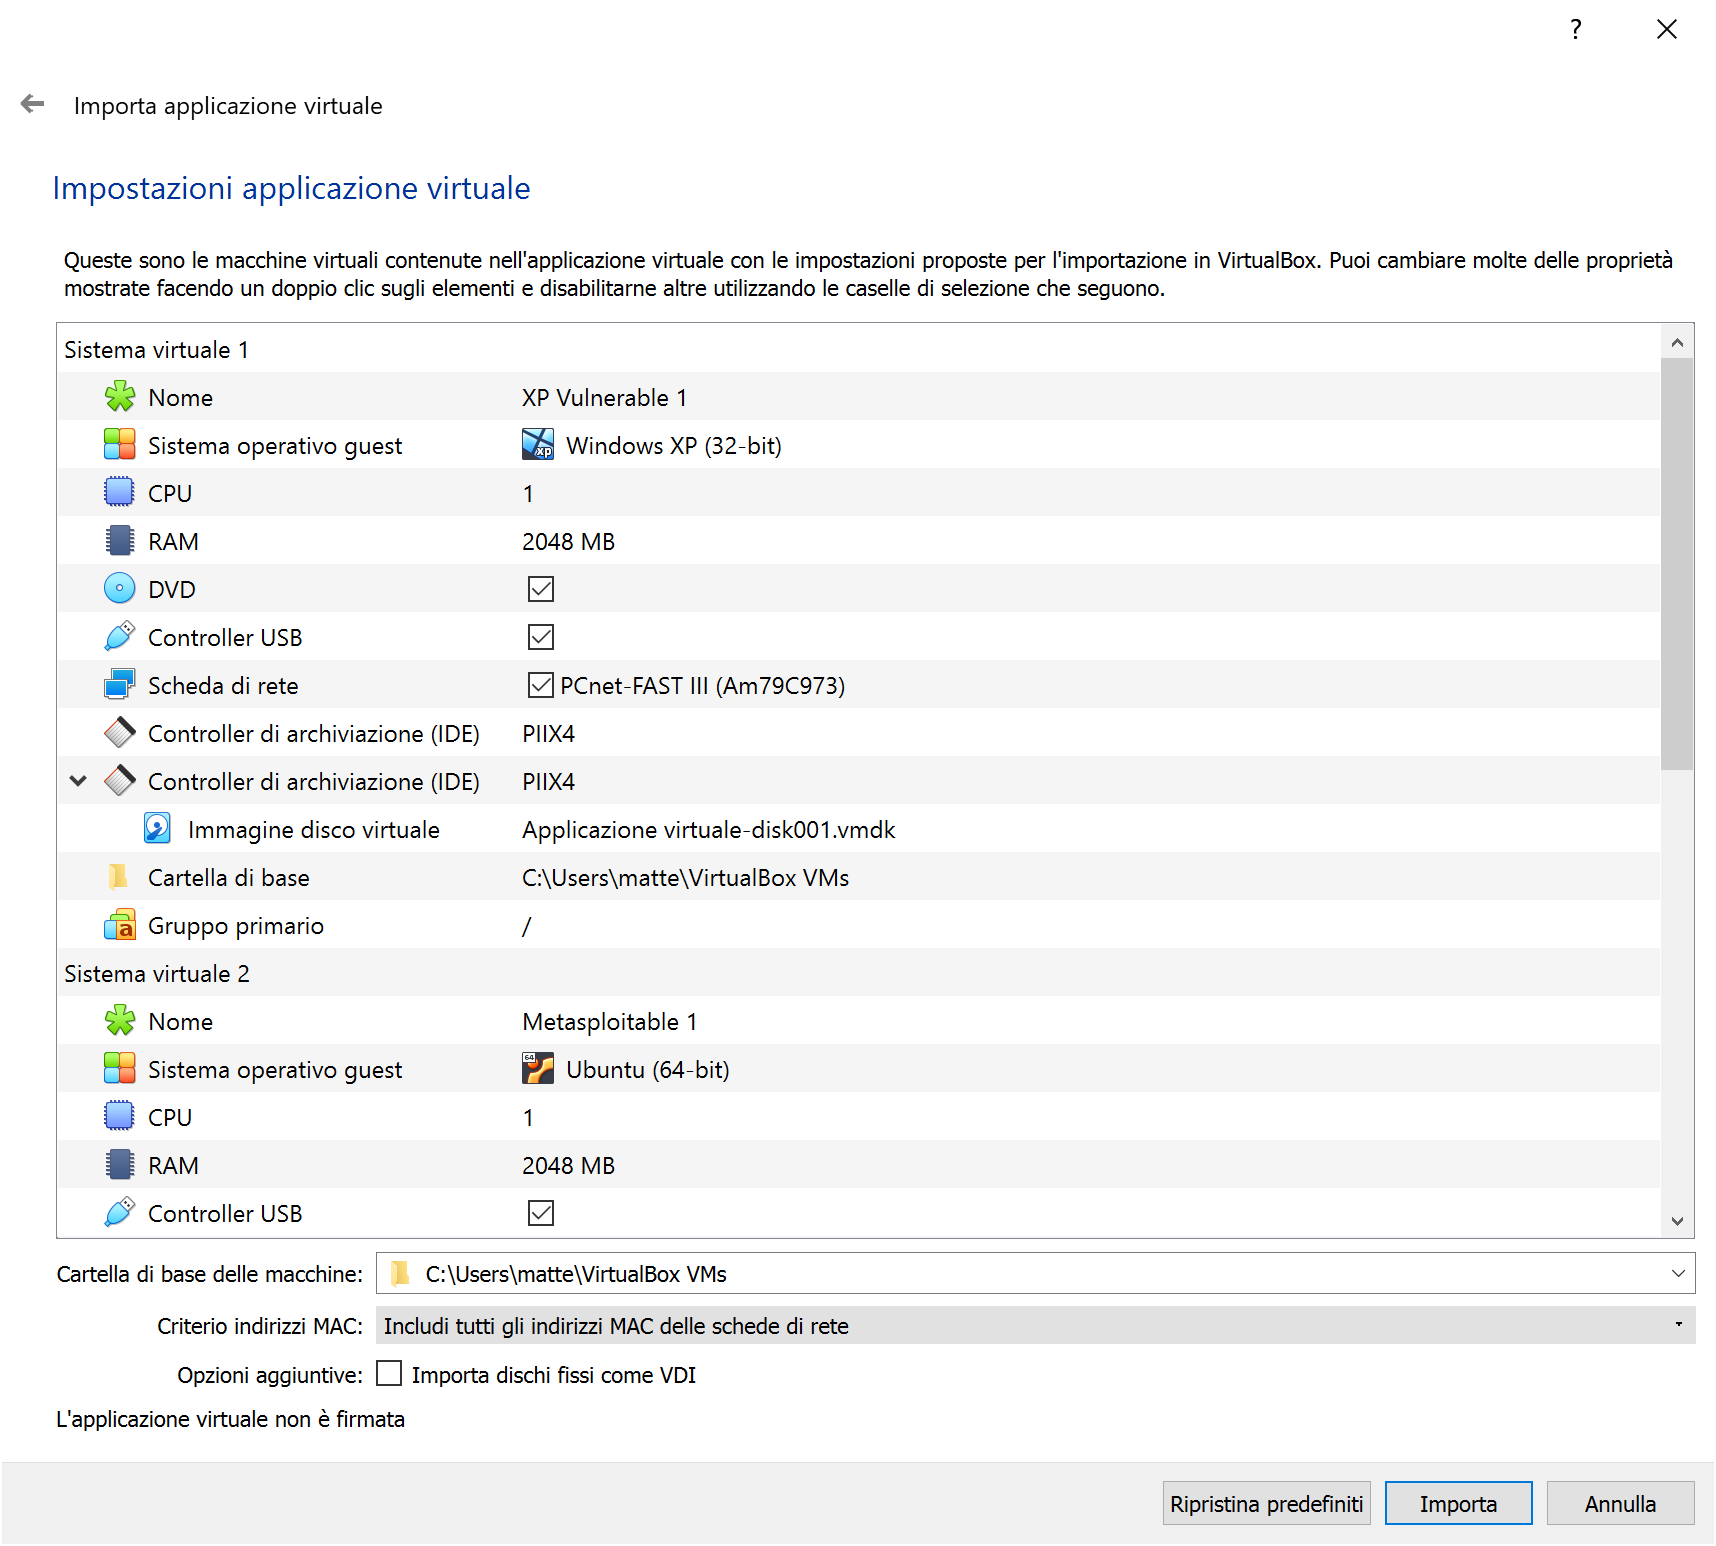
\includegraphics[width=0.7\textwidth]{../drawable/decorations/importing-screen.png}
    \caption{The final importing page}
    \label{fig:getting-started:import-screen}
\end{figure}

\begin{itemize}
    \item the MAC address dropdown menu is set to "Include all the MAC addresses"
    \item the saving location is set in a drive with at least \texttt{15 GB} of free space (\texttt{25 GB} recommended)
    \item there are three VMs to be imported: Windows XP, Metasploitable 1, Kali Linux-2021.1 1: the first two with 1 \texttt{vCPU}, the last with 2 \texttt{vCPU}, each one with \texttt{2048 MB} of RAM, a \texttt{vmdk} disk attached (with the USB controller set to on), and a network adapter.
\end{itemize}

If the requirements are unable to be satisfied by the host machine, you are free to reduce the RAM required by each machine by clicking it and editing it on the fly. Once the check is complete, please import the VMs and wait until all of them have been added to the list.

\subsubsection{Without the \texttt{ova} file}
\label{subsubsec:getting-started:without-ova}

The environment can be optionally recreated from scratch. First, VirtualBox must be installed along with the Oracle VM VirtualBox Extension Pack. Then, images for the three VMs must be retrieved and installed:

\begin{itemize}
    \item Kali Linux: downloadable from the offical website\footnote{\url{https://www.kali.org/downloads/}}
    \item Metasploitable 1: being a \texttt{EOL} product, can be retrieved from VulnHub\footnote{\url{https://www.vulnhub.com/entry/metasploitable-1,28/}}
    \item Windows XP: as it is not free software, it must be retrieved on one's own.
\end{itemize}

The Metasploitable machine is ready and does not need additional  modifications. The Windows XP machine is based on Windows XP SP2, and needs the following software to be installed:

\begin{itemize}
    \item \textbf{Adobe Reader} version \texttt{9.0.0} (to be used to execute the infected \texttt{PDF} exploit)
    \item \textbf{FreeSSHd} to offer \texttt{SSH} and \texttt{FTP} services (for remote management of the machine). The home directory for the \texttt{FTP} server has to be a shared folder.
    \item \textbf{Internet Information Services} installed (for the \texttt{TELNET} server)
\end{itemize}

The Kali Linux, depending on the flavor of the download, may or may not come with the Metasploit Framework installed, and additionally requires setting up the database. These steps can be found in Section \ref{subsec:getting-started:installing metasploit}.

Finally, remember to set up a virtual network bridge and to assign it to each VM's network interface in order to allow communication.

\subsection{Inspecting the environment}

Once the VMs are successfully deployed, we can proceed with the next step. First, start all of them and use the following credentials to log in once they have booted:

\begin{table}[htbp]
\centering
\begin{tabular}{|l|l|l|}
\hline 
Machine        & Username   & Password \\
\hline 
Kali Linux     & \texttt{kali}       & \texttt{kali}     \\
Metasploitable & \texttt{msfadmin}   & \texttt{msfadmin} \\
Windows XP     & \texttt{vulnerable} & \texttt{root}     \\
\hline
\end{tabular}
\end{table}

Then, open up a shell in each VM and verify the IPs (or set them, if you created them from scratch). They should be as in Figure \ref{fig:getting-started:network-conf}. Figure \ref{fig:getting-started:network-diagram} shows a simplified diagram of the obtained network.

\begin{figure}[htbp]
	\centering
	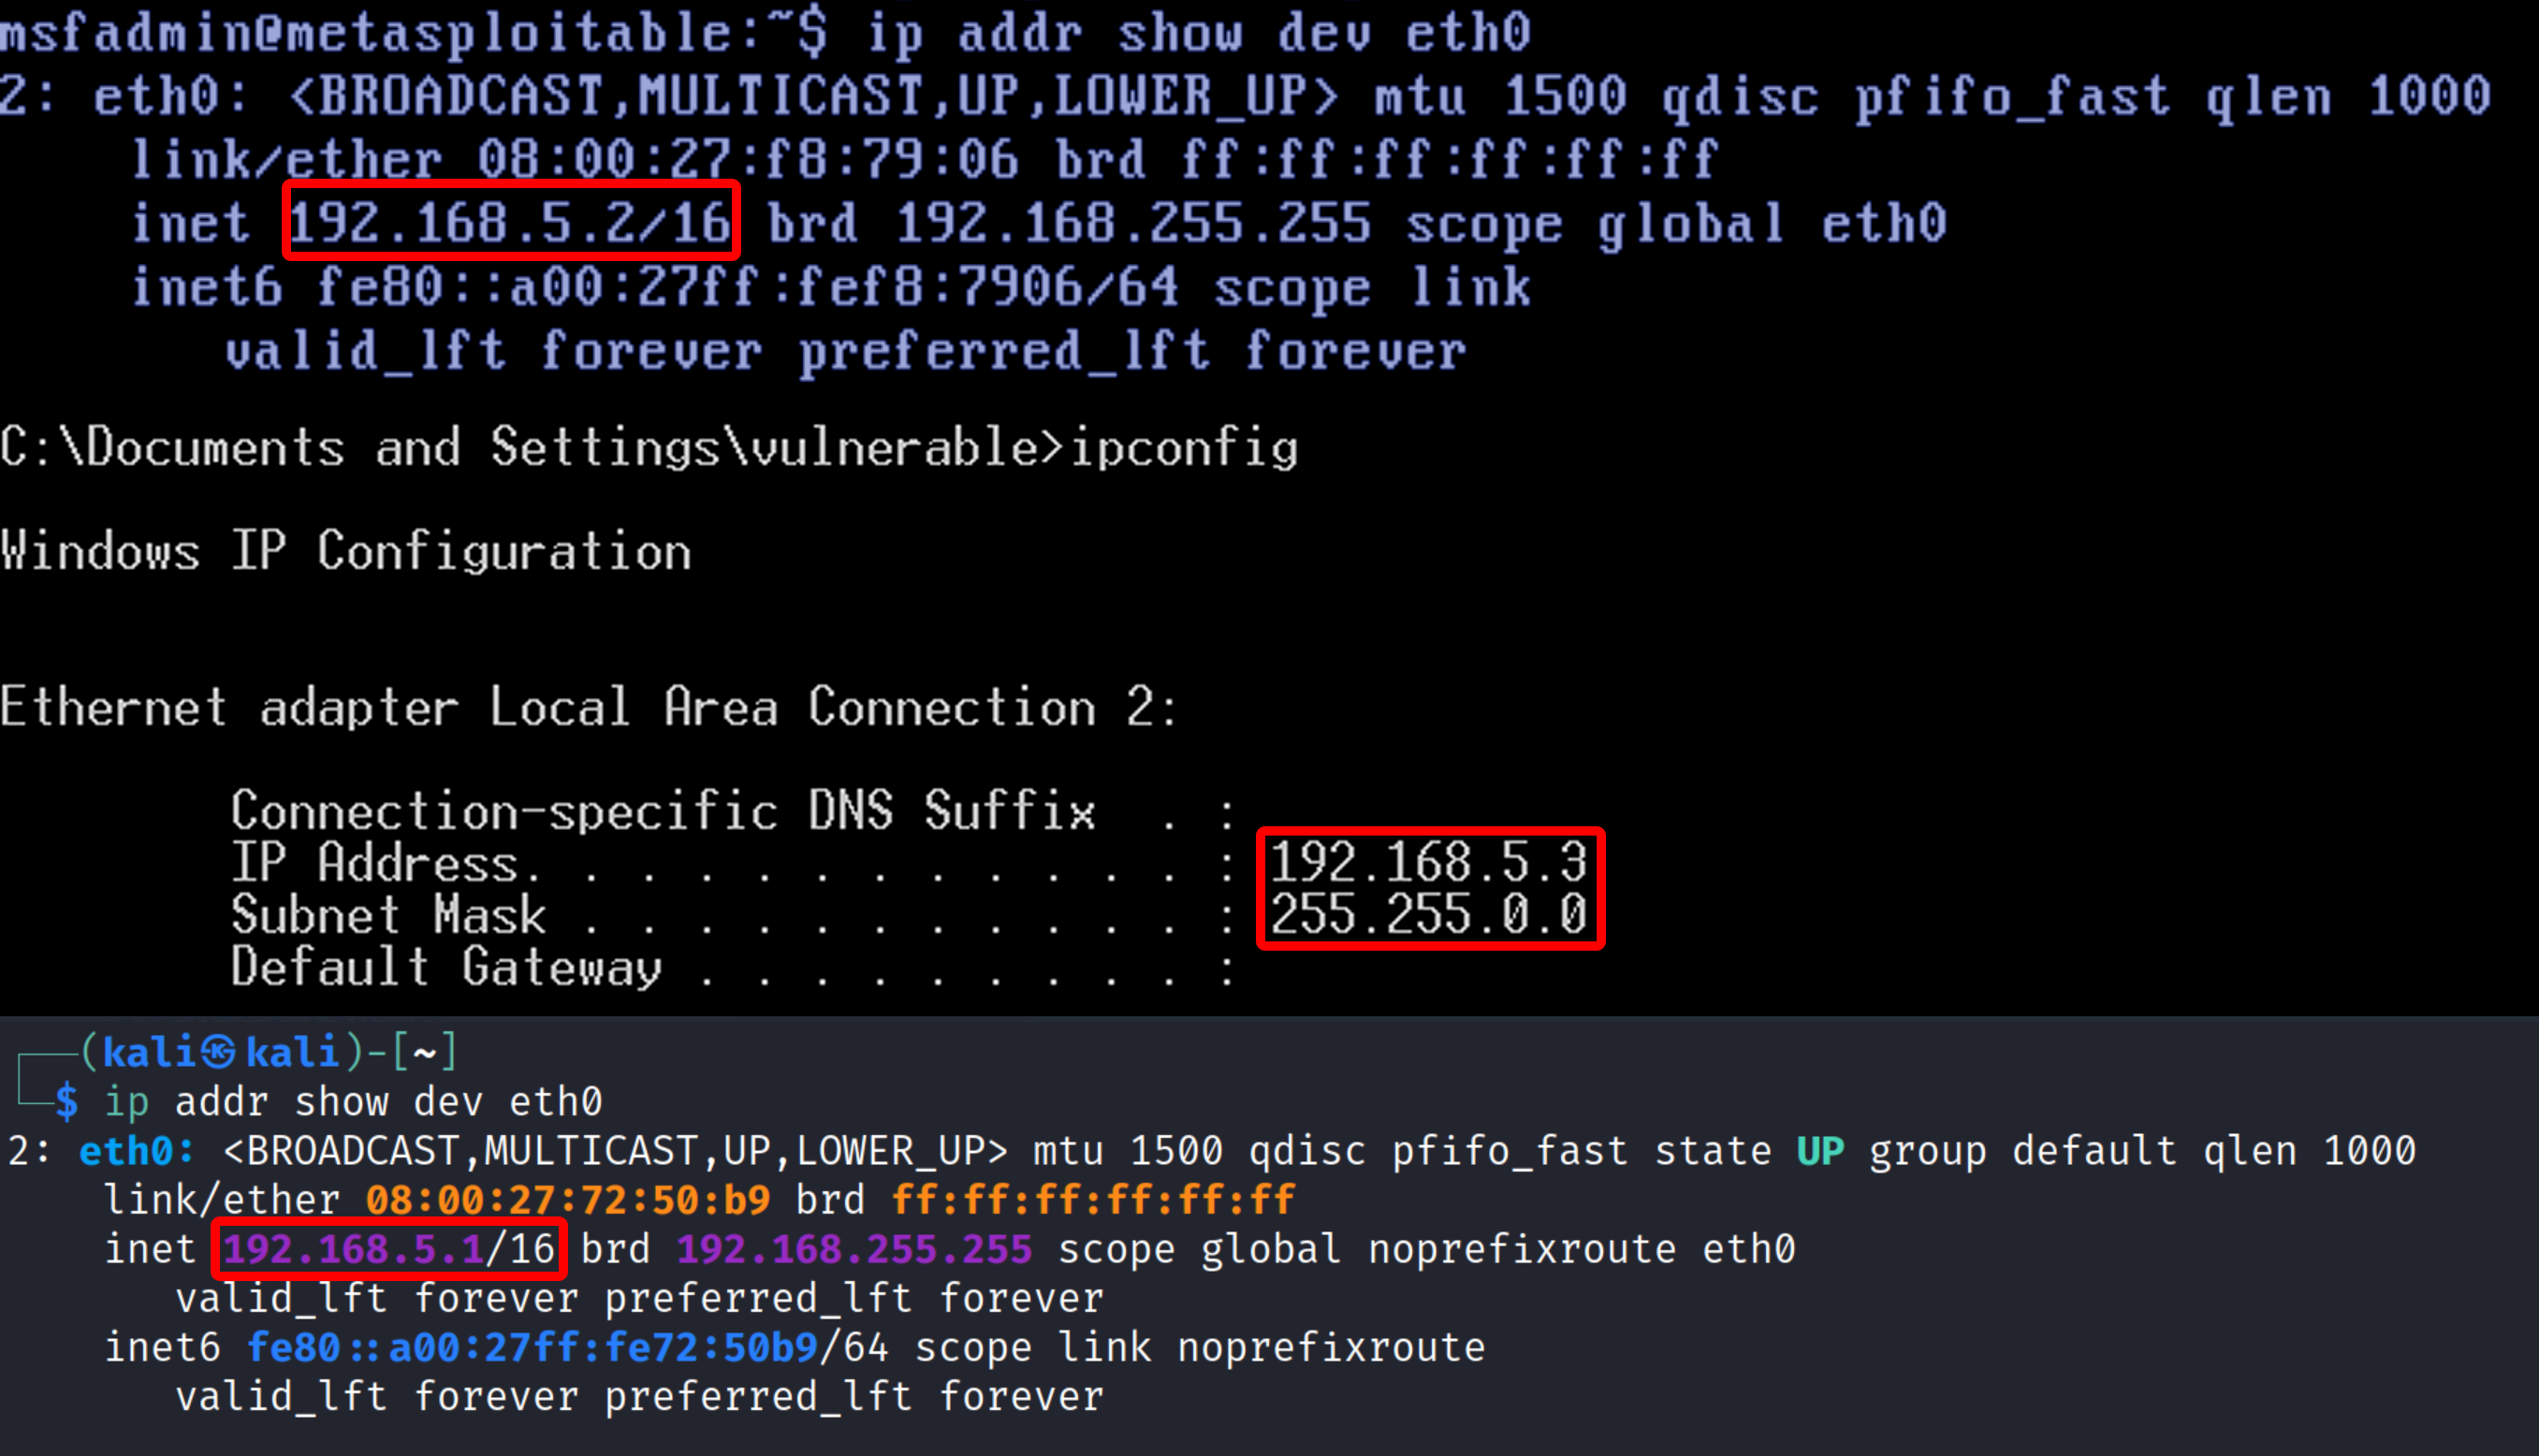
\includegraphics[width=\textwidth]{../drawable/preliminaries_screenshots/prel-ips.png}
    \caption{The network configuration for all VMs.}
    \label{fig:getting-started:network-conf}
\end{figure}

\begin{figure}[htbp]
	\centering
	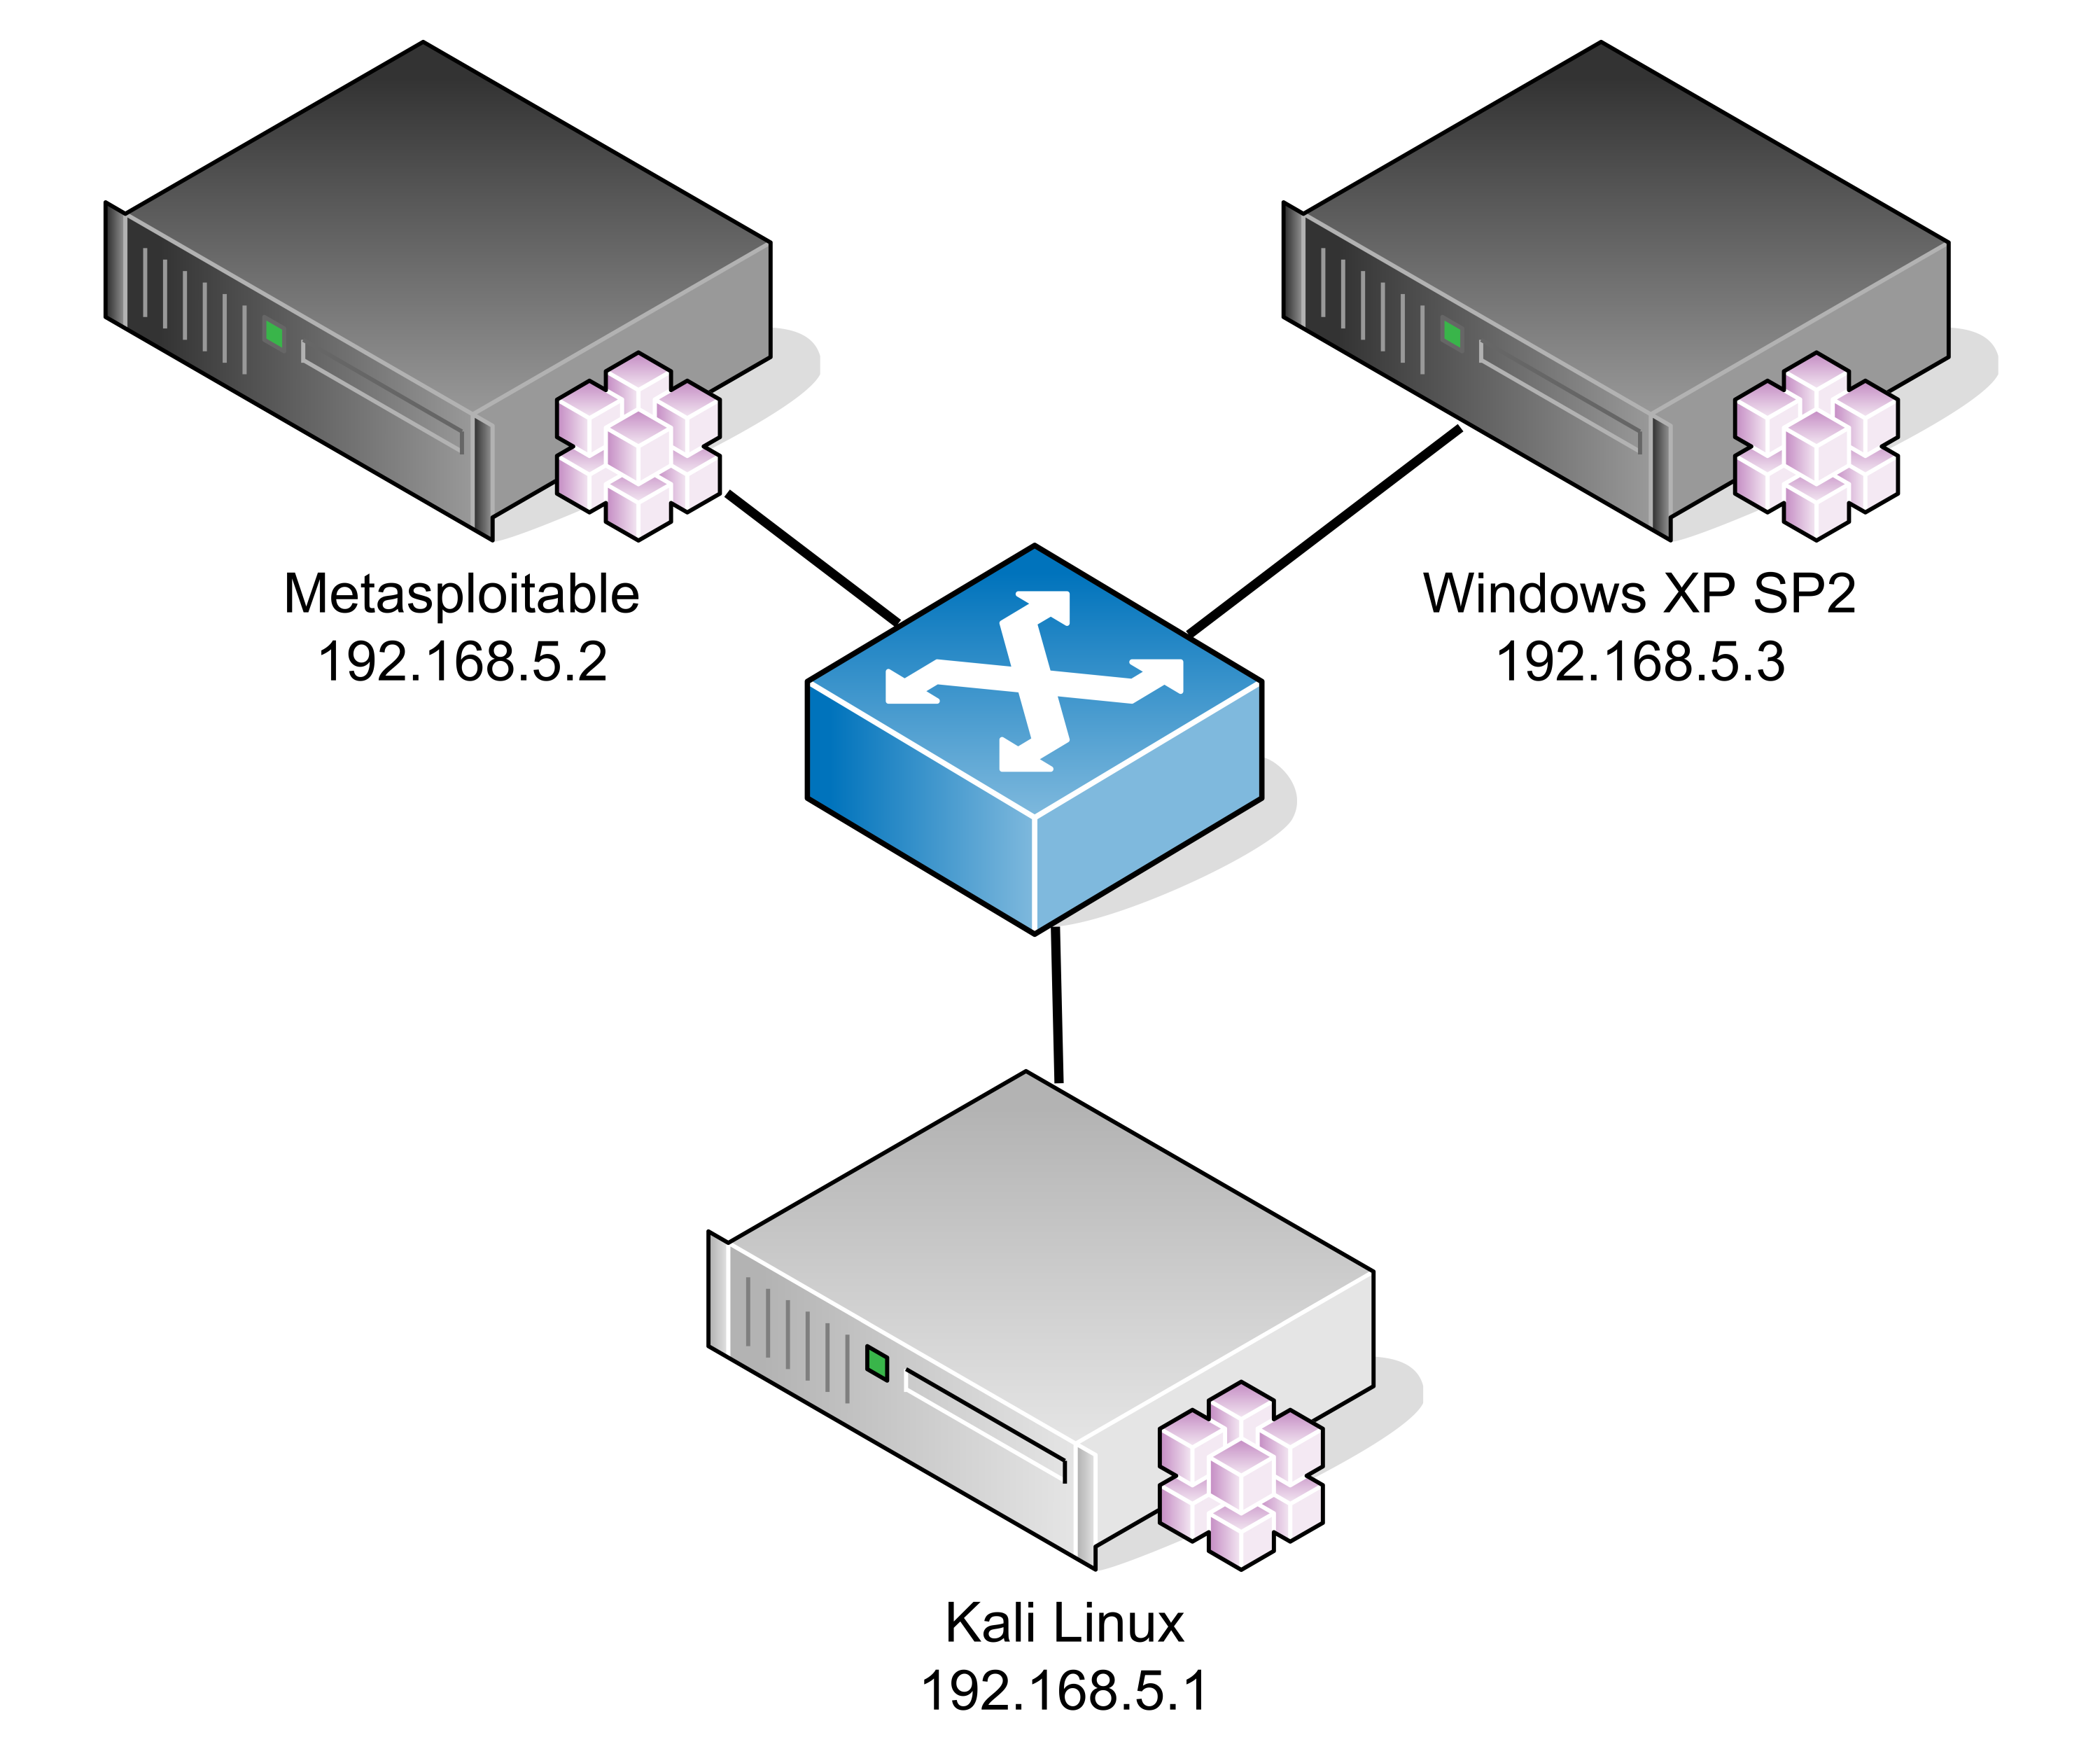
\includegraphics[width=0.4\textwidth]{../drawable/preliminaries_screenshots/prel-net.png}
    \caption{Diagram of the obtained network.}
    \label{fig:getting-started:network-diagram}
\end{figure}

\subsection{Installing Metasploit}
\label{subsec:getting-started:installing metasploit}

The following instructions are directly taken from the official Metasploit Framework page\footnote{\url{https://docs.rapid7.com/metasploit/installing-the-metasploit-framework/}}. Beginning from this section, code snippets shown in \hltexttt{dark\mbox{ }background} are intended as shell commands.\cite{online:msf-installation}

As Kali is a Linux distribution, we can proceed with the following command:

\begin{lstlisting}
curl "https://raw.githubusercontent.com/rapid7/metasploit-omnibus
    /master/config/templates/metasploit-framework-wrappers/
    msfupdate.erb" > msfinstall 
    && chmod 755 msfinstall 
    && ./msfinstall
\end{lstlisting}

We can then fire up \texttt{msfconsole}. Root privileges are recommended, as they will be needed in later exercises for both scanning and connection opening on well-known ports:

\begin{lstlisting}
sudo msfconsole
\end{lstlisting}

At startup, \texttt{msfconsole} will ask whether to set up a database. Insert \texttt{y} and let the console finalize the installation. If all goes well, inputting \texttt{db\_status} should yield:

\begin{lstlisting}
postgresql connected to msf
\end{lstlisting}

This means we're ready to get started with the basics of Metasploit.

\subsection{Commands}

The \texttt{msfconsole} is a full fledged shell with autocompletion and help pages. Inserting \hltexttt{?} or \hltexttt{help} will yield a long help page which covers all commands available for the user. For now, we will however focus on navigation and very basic usage.

As we said before, Metasploit's functionalities are logically divided into modules. \texttt{msfconsole} is packed with a powerful search tool which can index and retrieve modules very efficiently. To get started, one can write

\begin{lstlisting}
search eternalblue
\end{lstlisting}

in order to retrieve a full list of results of modules related to our query:

\begin{figure}[htbp]
	\centering
	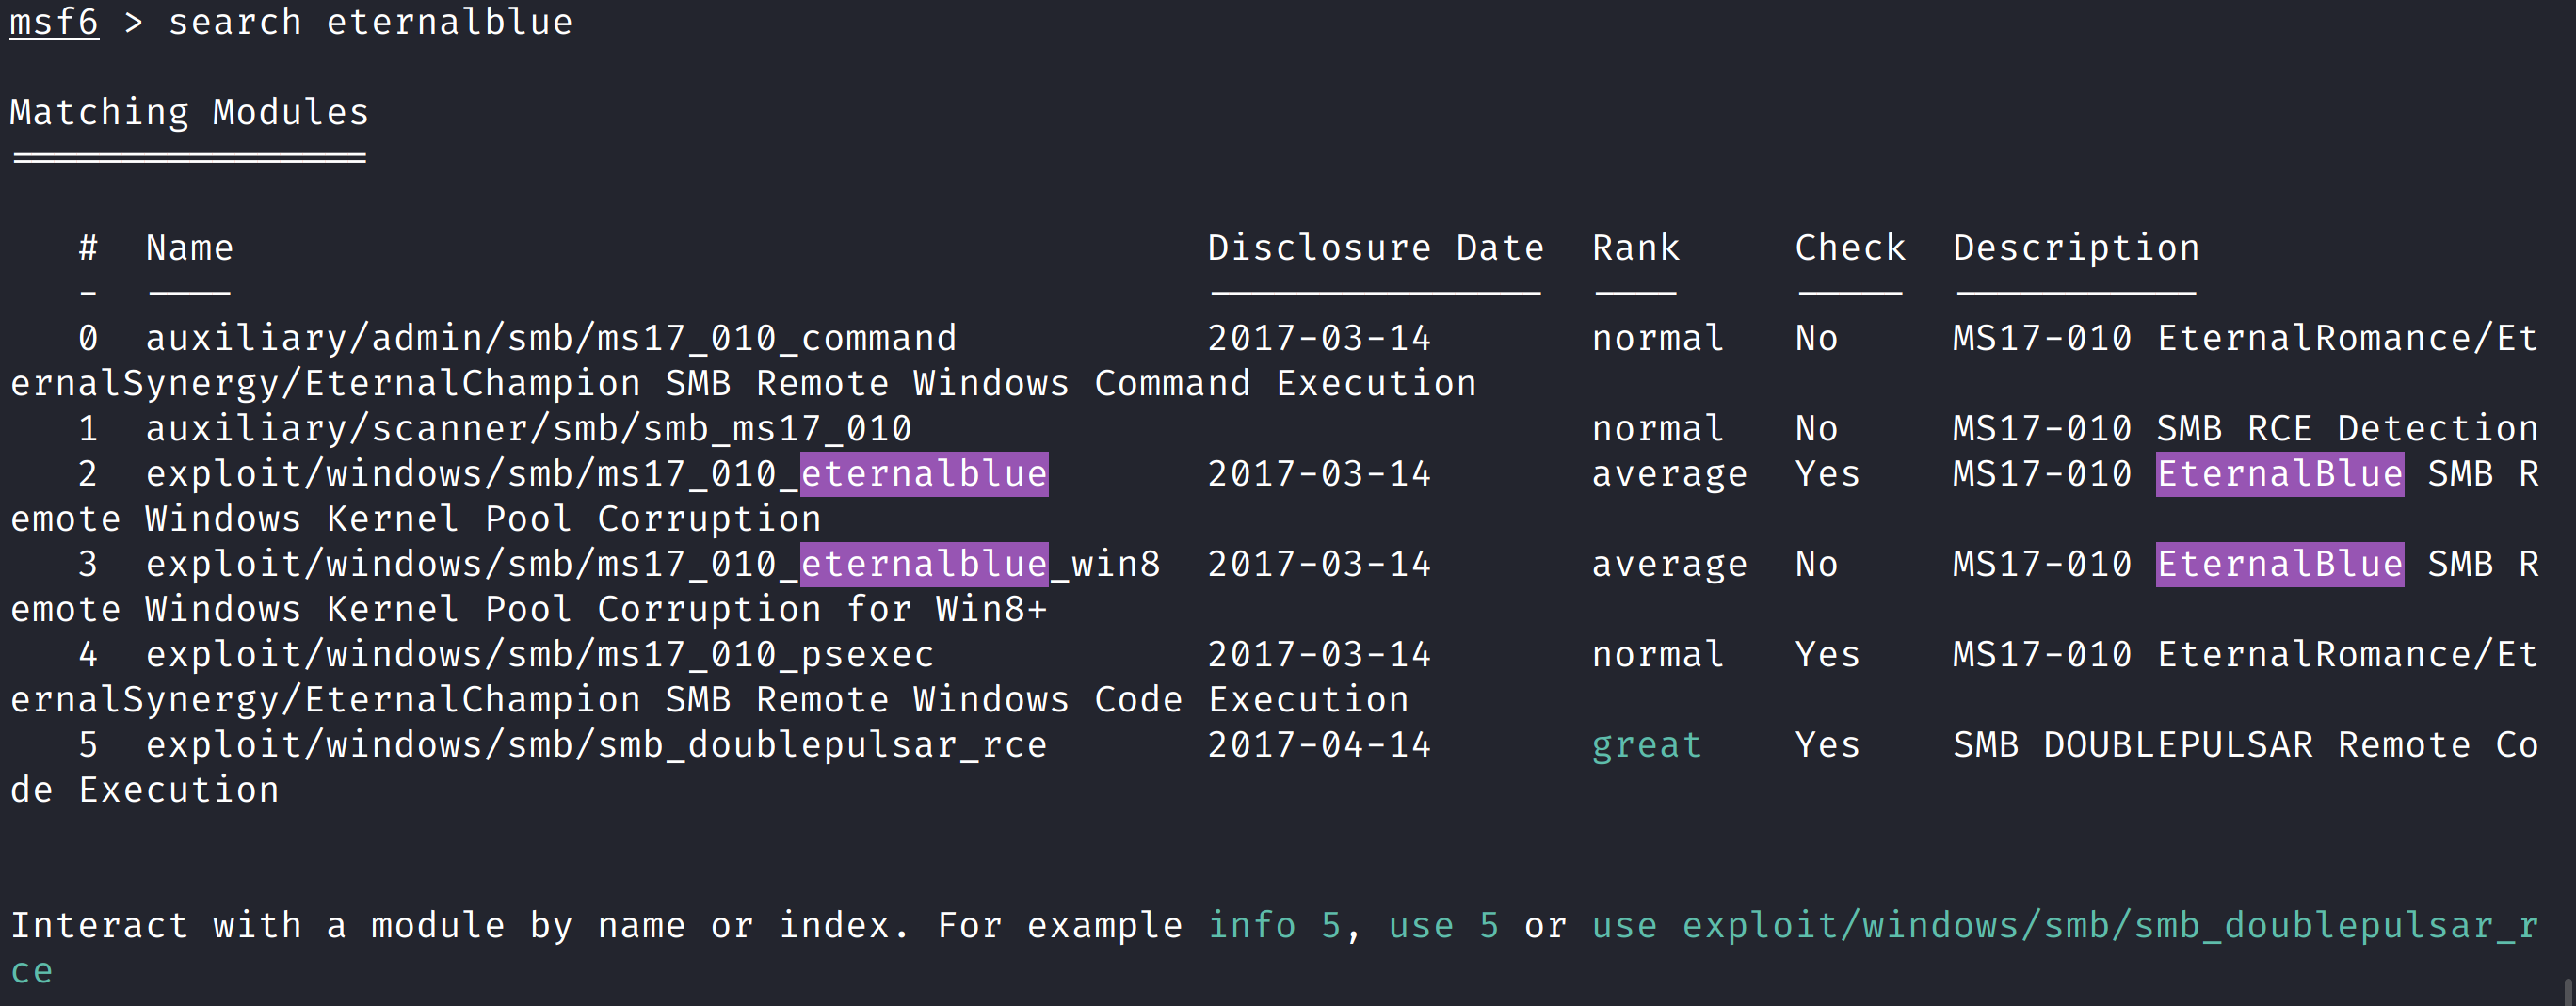
\includegraphics[width=\textwidth]{../drawable/preliminaries_screenshots/search-eternalblue.png}
    \caption{The results of a query in \texttt{msfconsole}}
    \label{fig:getting-started:query-search}
\end{figure}

Each module is sorted hierarchically by type, then platform, and then protocol. For example, we can inspect the infamous DoublePulsar exploit (listed as \texttt{exploit/windows/smb/smb\_doublepulsar\_rce}) by typing \hltexttt{info\mbox{ }5} - the index in the newly printed list - or just typing \hltexttt{info} followed by the module name. The console comes into help with autocompletion by tabbing.

Other important values shown and not shown in the table include:

\begin{itemize}
    \item the disclosure date (\texttt{date})
    \item the ranking (\texttt{ranking}), which provides details about the reliability and impact of an exploit on a target (ranging from Low to Excellent)
    \item the affected platform (\texttt{platform})
    \item the type (\texttt{type})
    \item the CVE ID if present (\texttt{cve})
\end{itemize}

Each of these values can be used against the search against in order to narrow down a search:

\begin{lstlisting}
search platform:windows description:acrobat
search cve:2021 type:exploit
search type:payload 
\end{lstlisting}

The amount of filters is vast. Typing \hltexttt{help\mbox{ }search} will provide more than adequate information for the matter.

Once a module has been selected, we can move into the next phase by typing \hltexttt{use} followed by the search index number or the name. The shell will react accordingly, switching modes (Figure \ref{fig:getting-started:using-module}).

\begin{figure}[htbp]
	\centering
	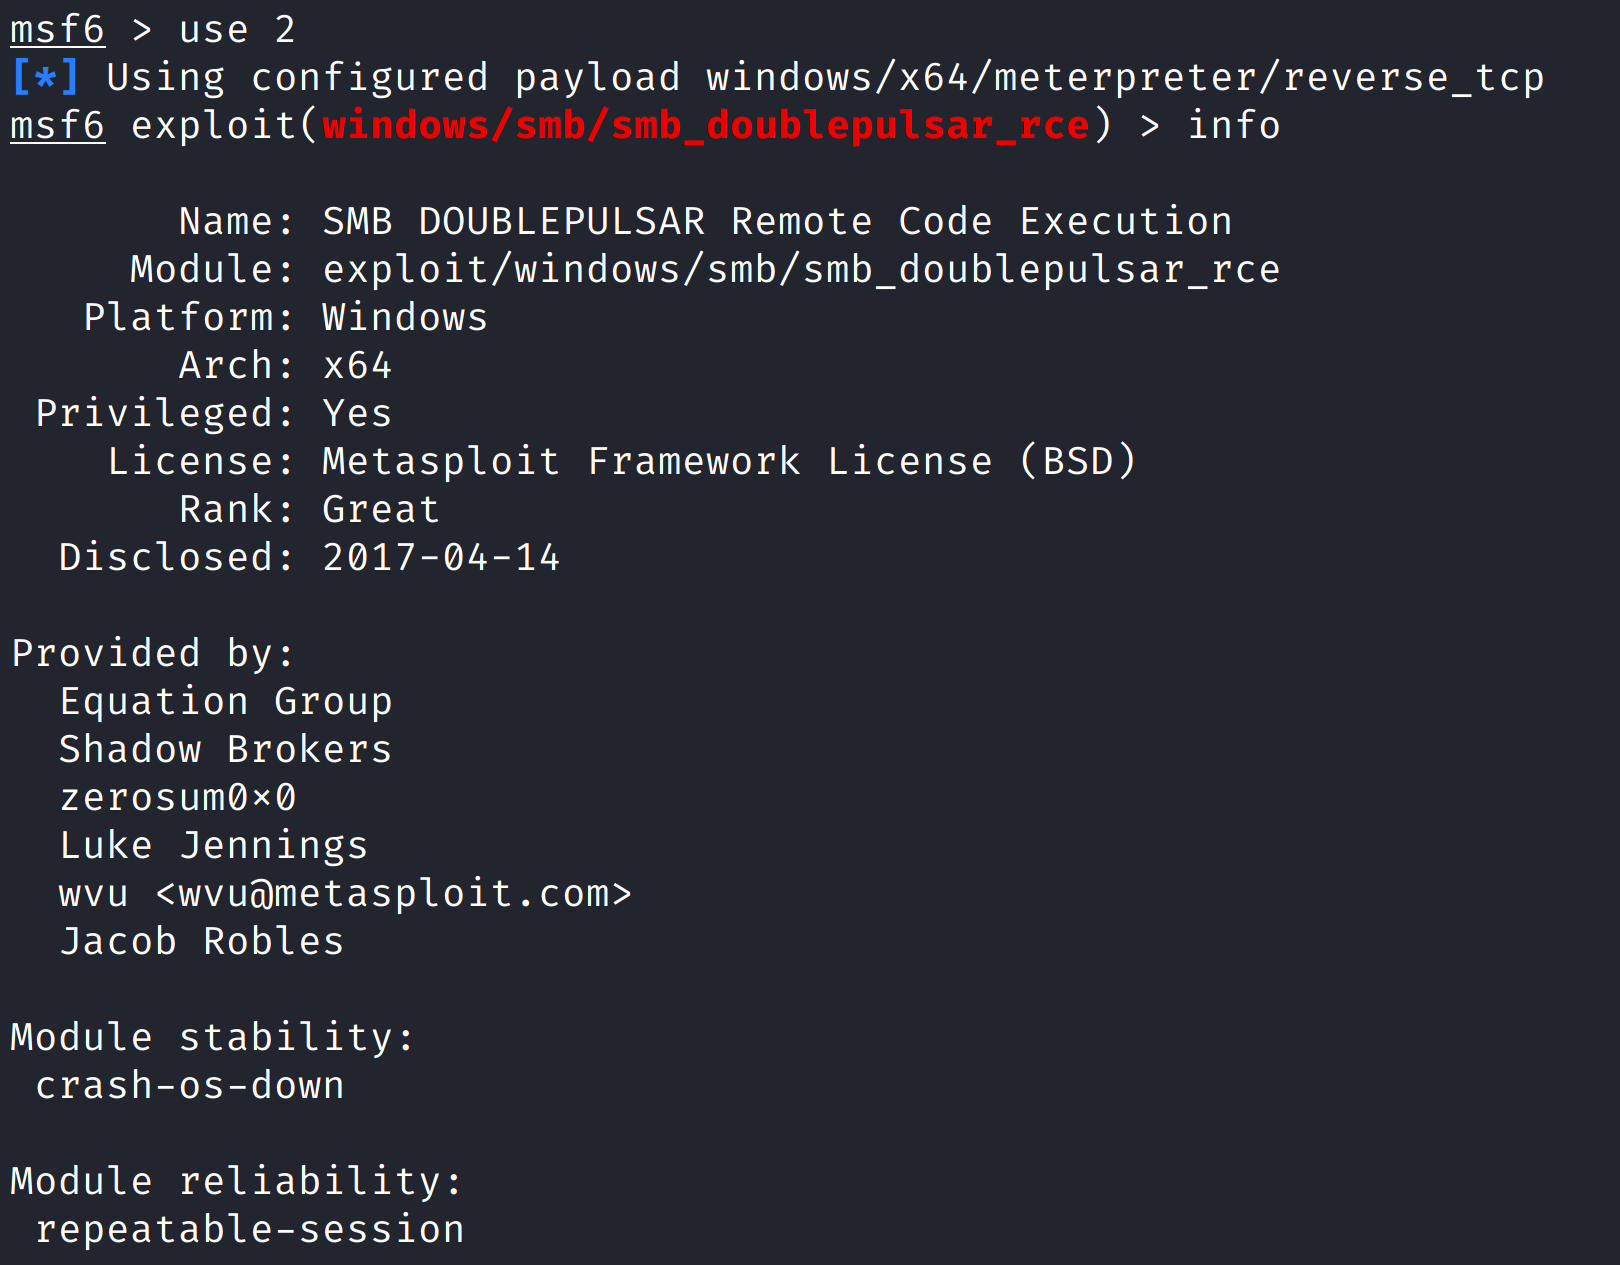
\includegraphics[width=0.7\textwidth]{../drawable/preliminaries_screenshots/info-eternalblue.png}
    \caption{Using a module in \texttt{msfconsole}: first, the mode switch, then an \hltexttt{info} command showing some information}
    \label{fig:getting-started:using-module}
\end{figure}

In this mode, we can type \hltexttt{info} to get a detailed report of the module at any time. Figure \ref{fig:getting-started:using-module} shows a small portion of the information about the DoublePulsar exploit we have chosen. Additionally, we can notice that when we typed \hltexttt{use\mbox{ }2} the Framework reminded us that the pre-configured payload was loaded (\texttt{windows/x64/meterpreter/reverse\_tcp}). Each exploit module has usually a default payload: we can surely change it with the following commands:

\begin{lstlisting}
show payloads
set payload [...]
\end{lstlisting}

It must be reminded that payloads are to be set only in case of exploit modules. In either case, we can have a glance at all the options of the module with \hltexttt{show\mbox{ }options}. Each one of them can be then \hltexttt{set} or \hltexttt{\mbox{unset}} with the homonymous commands.

\begin{figure}[htbp]
	\centering
	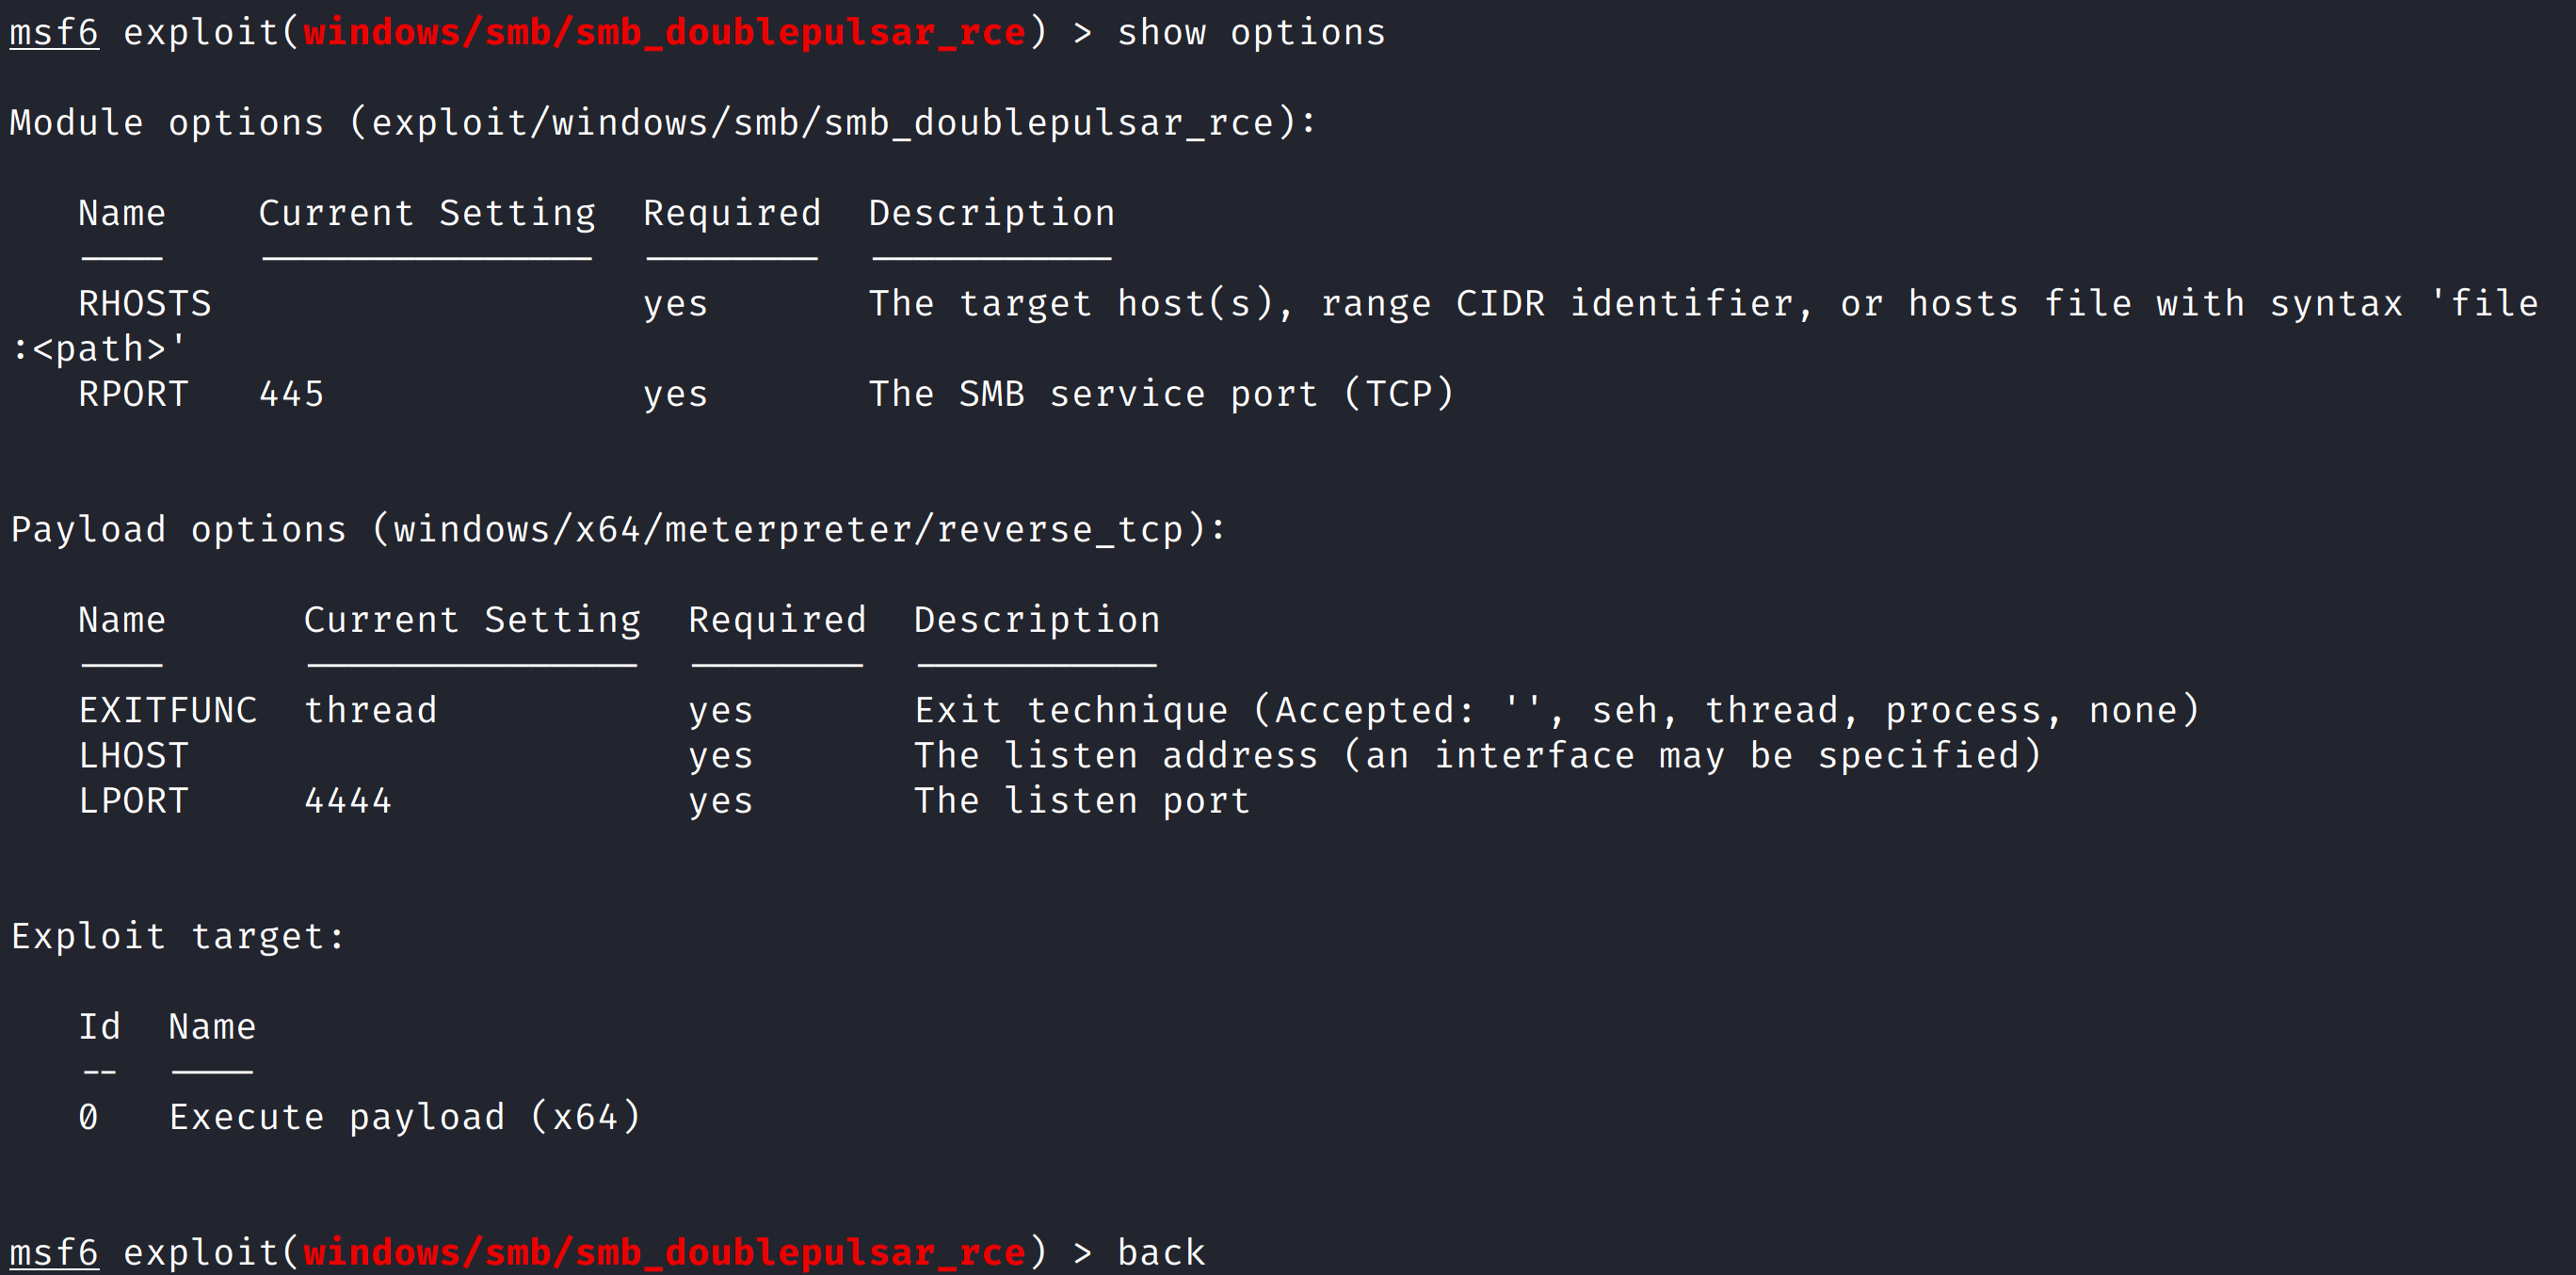
\includegraphics[width=\textwidth]{../drawable/preliminaries_screenshots/options-eternalblue.png}
    \caption{Showing a module's options, and going \hltexttt{back}}
    \label{fig:getting-started:options-back}
\end{figure}


Once we're set, we can mount the attack (in case of an exploit) with the \hltexttt{\mbox{exploit}} command, or run the module with \hltexttt{run}. For now, however, we'll just go \hltexttt{back} once to the main menu (Figure \ref{fig:getting-started:options-back}).

We conclude this introduction with a quick look at some supplementary commands:

\begin{itemize}
    \item \hltexttt{edit} - brings up the system textedit program to edit a particular file or, if run within a module, the module itself.
    \item \hltexttt{grep} - works exactly as its Unix counterpart (Warning! Pipes do not work within \texttt{msfconsole}. Use \texttt{grep} followed by the required command).
    \item \hltexttt{irb} - starts a Ruby shell, within the context of the current module.
    \item \hltexttt{jobs} - lists active jobs such as ongoing exploits.
    \item \hltexttt{kill} - shuts down an ongoing activity.
    \item \hltexttt{\mbox{sessions}} - shows currently open connections. Will be used in later exercises.
\end{itemize}

\clearpage